%%%%%%%%%%%%%%%%%%%%%%%%%%%%%%%%%%%%%%%%%%%%%%%%%%%%%%%%%%%%%%%%%%%%%%%%%%
%                                                                        %
%                            INTRODUCTION                                %
%                                                                        %
%%%%%%%%%%%%%%%%%%%%%%%%%%%%%%%%%%%%%%%%%%%%%%%%%%%%%%%%%%%%%%%%%%%%%%%%%%
\subsection*{}
\begin{frame}{Introduction}
  \large
  \centering{Will a candidate detector work?}
  \vspace{1cm}
  \normalsize
  \begin{itemize}
    \item Modeling is needed to simulate large area plastic
    \item MCNPX is a well validated transport code
    \begin{itemize}
        \item MCNPX is a Monte Carlo based
        \item MCNPX has drawbacks with energy deposition
    \end{itemize}
    \item Previous work has shown that it is possible to model detector neutronics with MCNPX
  \end{itemize}
\end{frame}
%%%%%%%%%%%%%%%%%%%%%%%%%%%%%%%%%%%%%%%%%%%%%%%%%%%%%%%%%%%%%%%%%%%%%%%%%%
\begin{frame}{Multi Film Model}
	\begin{figure}
    \vspace*{-9cm}
    \begin{subfigure}[b]{0.47\textwidth}
      \centering
      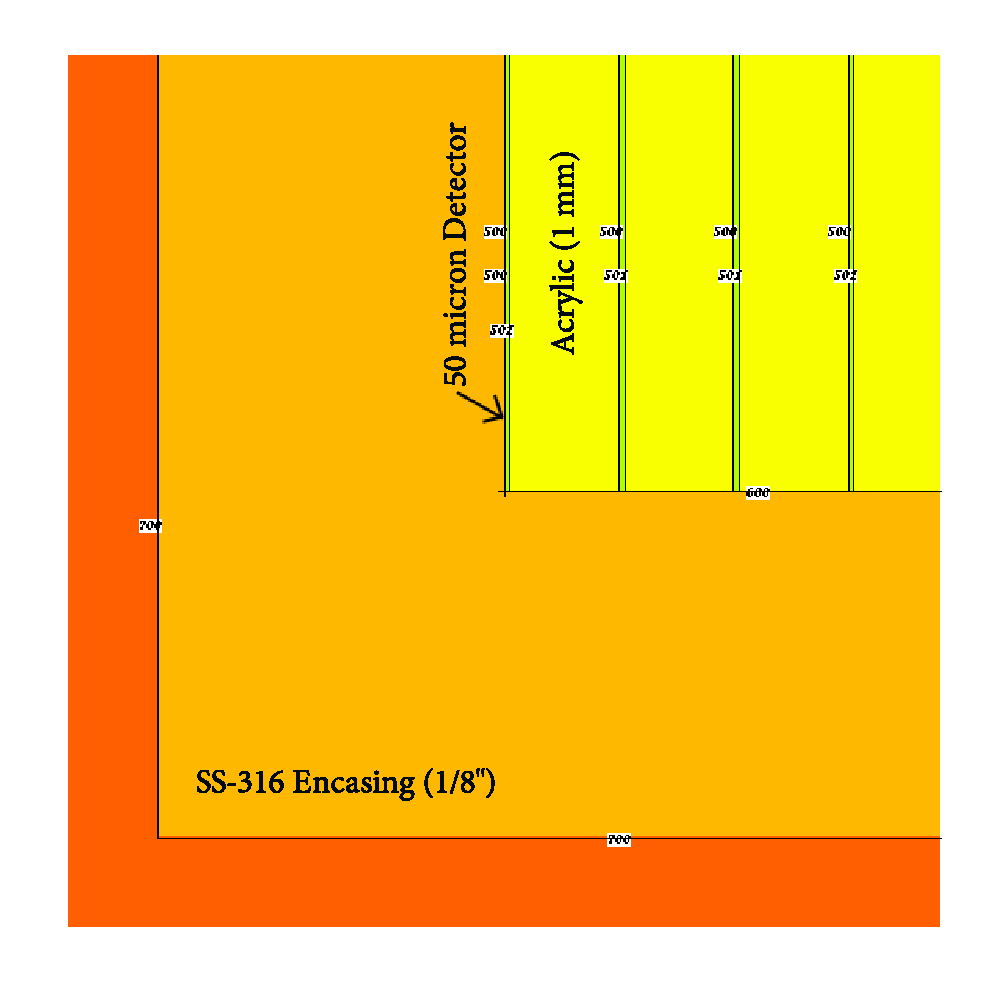
\includegraphics[width=\textwidth]{Multi_120Layers.eps}
      \caption{Simulated RPM8 Detector (120 layers)}
    \end{subfigure}
    ~
    \begin{subfigure}[b]{0.47\textwidth}
      \centering
      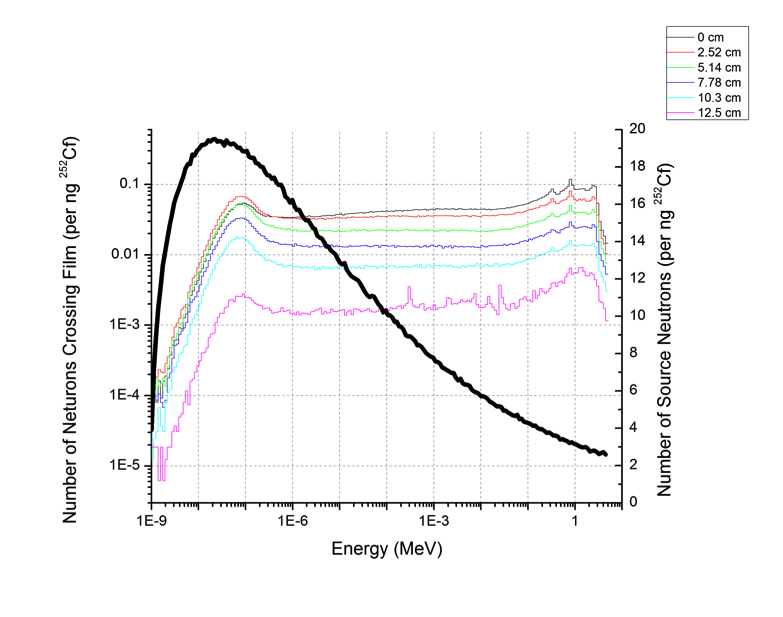
\includegraphics[width=2\textwidth]{Spectra_Layered.eps}
      \caption{Source and Incident Spectra}
    \end{subfigure}
	\end{figure}
\end{frame}
%%%%%%%%%%%%%%%%%%%%%%%%%%%%%%%%%%%%%%%%%%%%%%%%%%%%%%%%%%%%%%%%%%%%%%%%%%
\begin{frame}{Opportunities for Optimization}
  \begin{columns}[onlytextwidth]
    \begin{column}{0.45\textwidth}
    \begin{itemize}
      \item Neutron absorber loading of the film
      \item Thickness of the film
      \item Geometry of the film
      \item Placement of the films
    \end{itemize}
    \end{column}
    \begin{column}{0.45\textwidth}
      \begin{figure}
        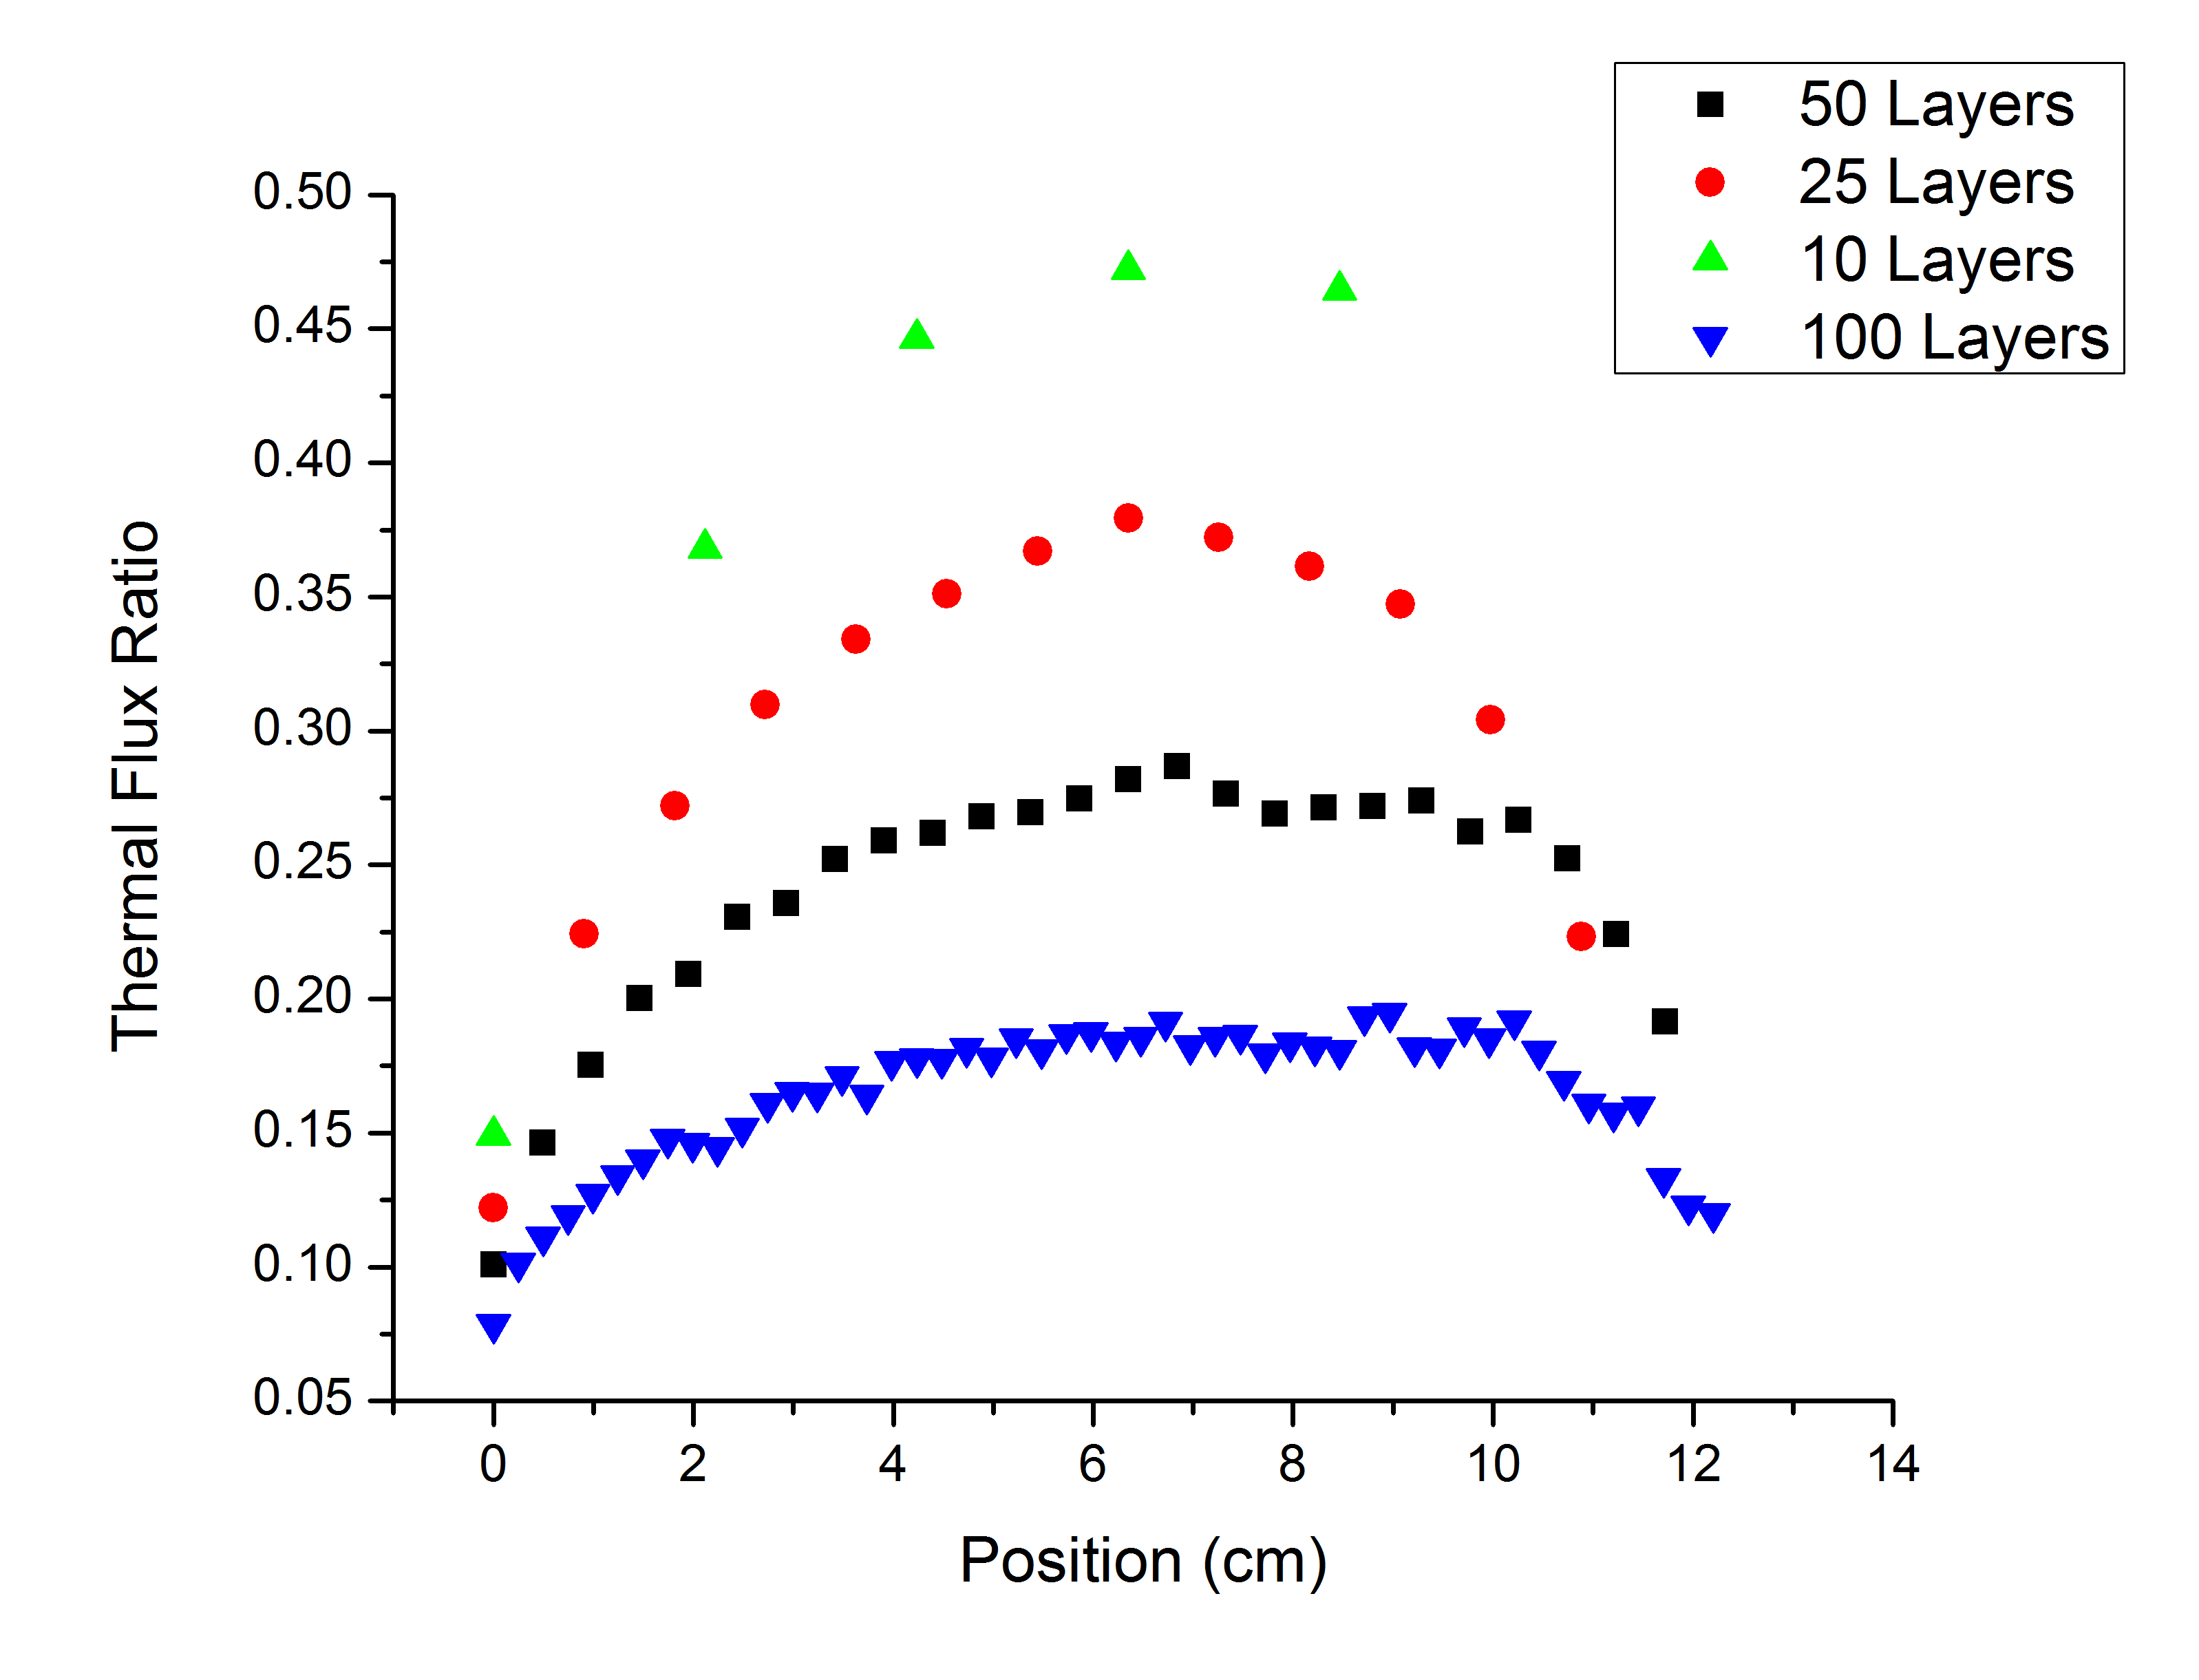
\includegraphics[width=\textwidth]{ThermalFluxRatioAltLayers}
      \end{figure}
    \end{column}
  \end{columns}
\end{frame}
%%%%%%%%%%%%%%%%%%%%%%%%%%%%%%%%%%%%%%%%%%%%%%%%%%%%%%%%%%%%%%%%%%%%%%%%%%
%                                                                        %
%                             PROPOSED WORK                              %
%                                                                        %
%%%%%%%%%%%%%%%%%%%%%%%%%%%%%%%%%%%%%%%%%%%%%%%%%%%%%%%%%%%%%%%%%%%%%%%%%%
\subsection{Proposed Work}
\begin{frame}{Proposed Work}
  \large
  \textbf{Optimization of the film placement}
  \normalsize
  \begin{itemize}
    \item Focus on minimizing amount of \iso[6]{Li} while meeting criteria
    \begin{itemize}
      \item Search the parameter space of possible detector designs
      \item Study effects of self-shielding and different geometries
    \end{itemize}
  \end{itemize}
\textbf{What do we mean by best?}
\begin{itemize}
	\small
  \item Count rate? 
  \item Light output?
	\item Lowest cost / fabrication ease?
\end{itemize}
\textbf{The design parameters were then:}
\begin{itemize}
	\small
  \item The detector material
  \item The thickness of the detector material
  \item The spacing of detector layers
\end{itemize}
\end{frame}
%%%%%%%%%%%%%%%%%%%%%%%%%%%%%%%%%%%%%%%%%%%%%%%%%%%%%%%%%%%%%%%%%%%%%%%%%%
%                                                                        %
%                               METHODS                                  %
%                                                                        %
%%%%%%%%%%%%%%%%%%%%%%%%%%%%%%%%%%%%%%%%%%%%%%%%%%%%%%%%%%%%%%%%%%%%%%%%%%
\subsection{Methods}
\begin{frame}[fragile]
\frametitle{Neutron Interaction Rate}
	\tiny
	\newtheorem{thm11}{Interaction Rate}
	\begin{thm11}<1->
		$$Q = C \int {\Phi(E) R_m(E) dE }$$
	where:
	\begin{itemize}
		\item $C$ is a scalar normalization (density)
		\item $R_m(E)$ is the response function
		\item $\Phi(E)$ is the neutron flux
	\end{itemize}
	\end{thm11}
Accomplished using a F4 tally with multiplier
\tiny
\begin{lstlisting}
c -------- Interaction Rate Tallies -------------
FC154 (n,t) Reactions in Detector
F154:n (601<610) (602<610) (603<610) (604<610) T
FM154 -1 3 105
\end{lstlisting}
\end{frame}
%%%%%%%%%%%%%%%%%%%%%%%%%%%%%%%%%%%%%%%%%%%%%%%%%%%%%%%%%%%%%%%%%%%%%%%%%%
\begin{frame}[fragile]{Gigantic Genome Geometries}
\label{GAMethod}
Genome Bit-String Representation
\begin{itemize}
  \item Divide the RPM8 width into even slices
  \item Compact representation of geometry, suitable for GA
  \item \verb+1+ - represents a detector assembly slice
  \item \verb+0+ - represents a moderator slice
  \item Example: \verb+001000+
  \begin{itemize}
    \item Each slice is \SI{2.12}{\centi\meter}
    \item Two slices of moderator, followed by one assembly slice followed by three additional slices of moderator
  \end{itemize}
\end{itemize}
\hyperlink{GAMethodExtended}{\beamerbutton{Detailed GA Introduction}}
\end{frame}
%%%%%%%%%%%%%%%%%%%%%%%%%%%%%%%%%%%%%%%%%%%%%%%%%%%%%%%%%%%%%%%%%%%%%%%%%%
\begin{frame}{Example Geometry}
\begin{columns}[onlytextwidth]
  \begin{column}{0.45\textwidth}
    \small
    \begin{itemize}
      \item Population of candidate solutions is evolved toward better solutions
      \item Each candidate has properties that can be mutated and altered
      \item Traditionally solutions are represented as bit strings or trees
    \end{itemize}
    \end{column}
  \begin{column}{0.45\textwidth}
    \begin{figure}
		\tiny
    \end{figure}
  \end{column}
\end{columns}
\hyperlink{GAMethodExtended}{\beamerbutton{Detailed GA Introduction}}
\end{frame}
%%%%%%%%%%%%%%%%%%%%%%%%%%%%%%%%%%%%%%%%%%%%%%%%%%%%%%%%%%%%%%%%%%%%%%%%%%
%                                                                        %
%                          PRELIMARY RESULTS                             %
%                                                                        %
%%%%%%%%%%%%%%%%%%%%%%%%%%%%%%%%%%%%%%%%%%%%%%%%%%%%%%%%%%%%%%%%%%%%%%%%%%
\subsection{Preliminary Results}
%%%%%%%%%%%%%%%%%%%%%%%%%%%%%%%%%%%%%%%%%%%%%%%%%%%%%%%%%%%%%%%%%%%%%%%%%%
\begin{frame}{Optimal Geometries Rendered}
\begin{figure}
    \centering
    \begin{subfigure}[b]{0.45\textwidth}
        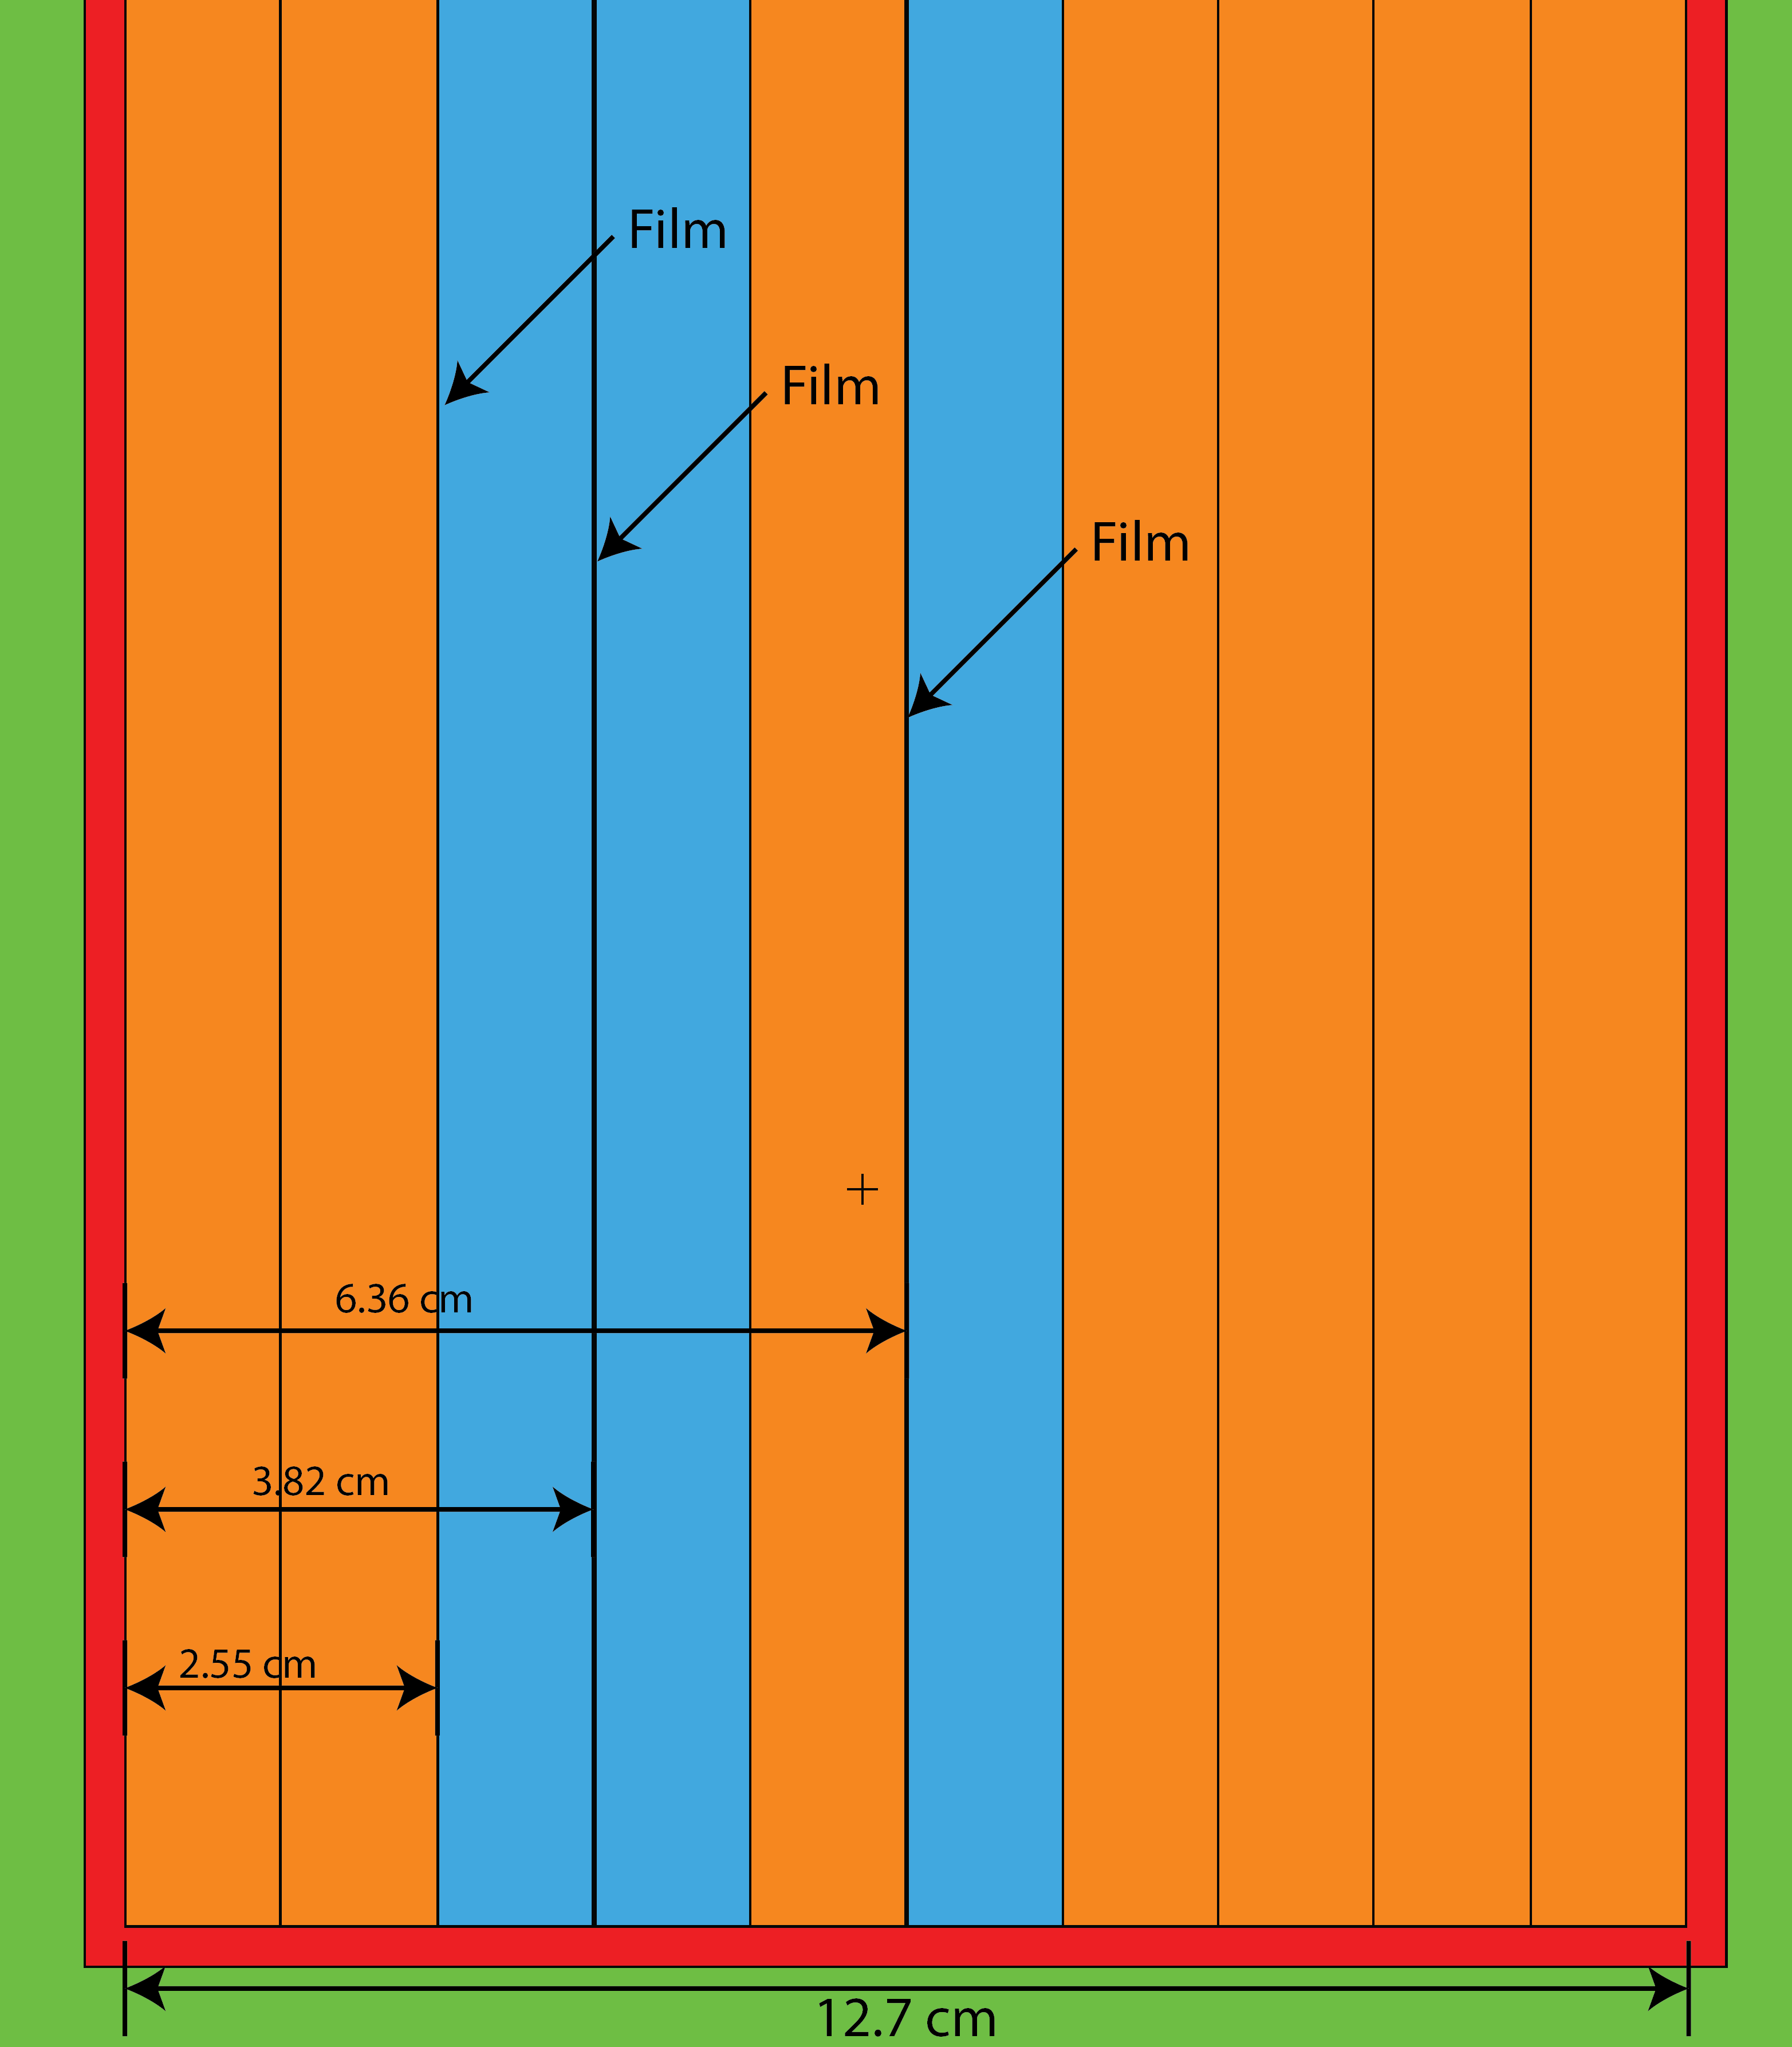
\includegraphics[width=\textwidth]{RPM8OptLayered_25cps}
    \end{subfigure}%
    ~
    \begin{subfigure}[b]{0.45\textwidth}
        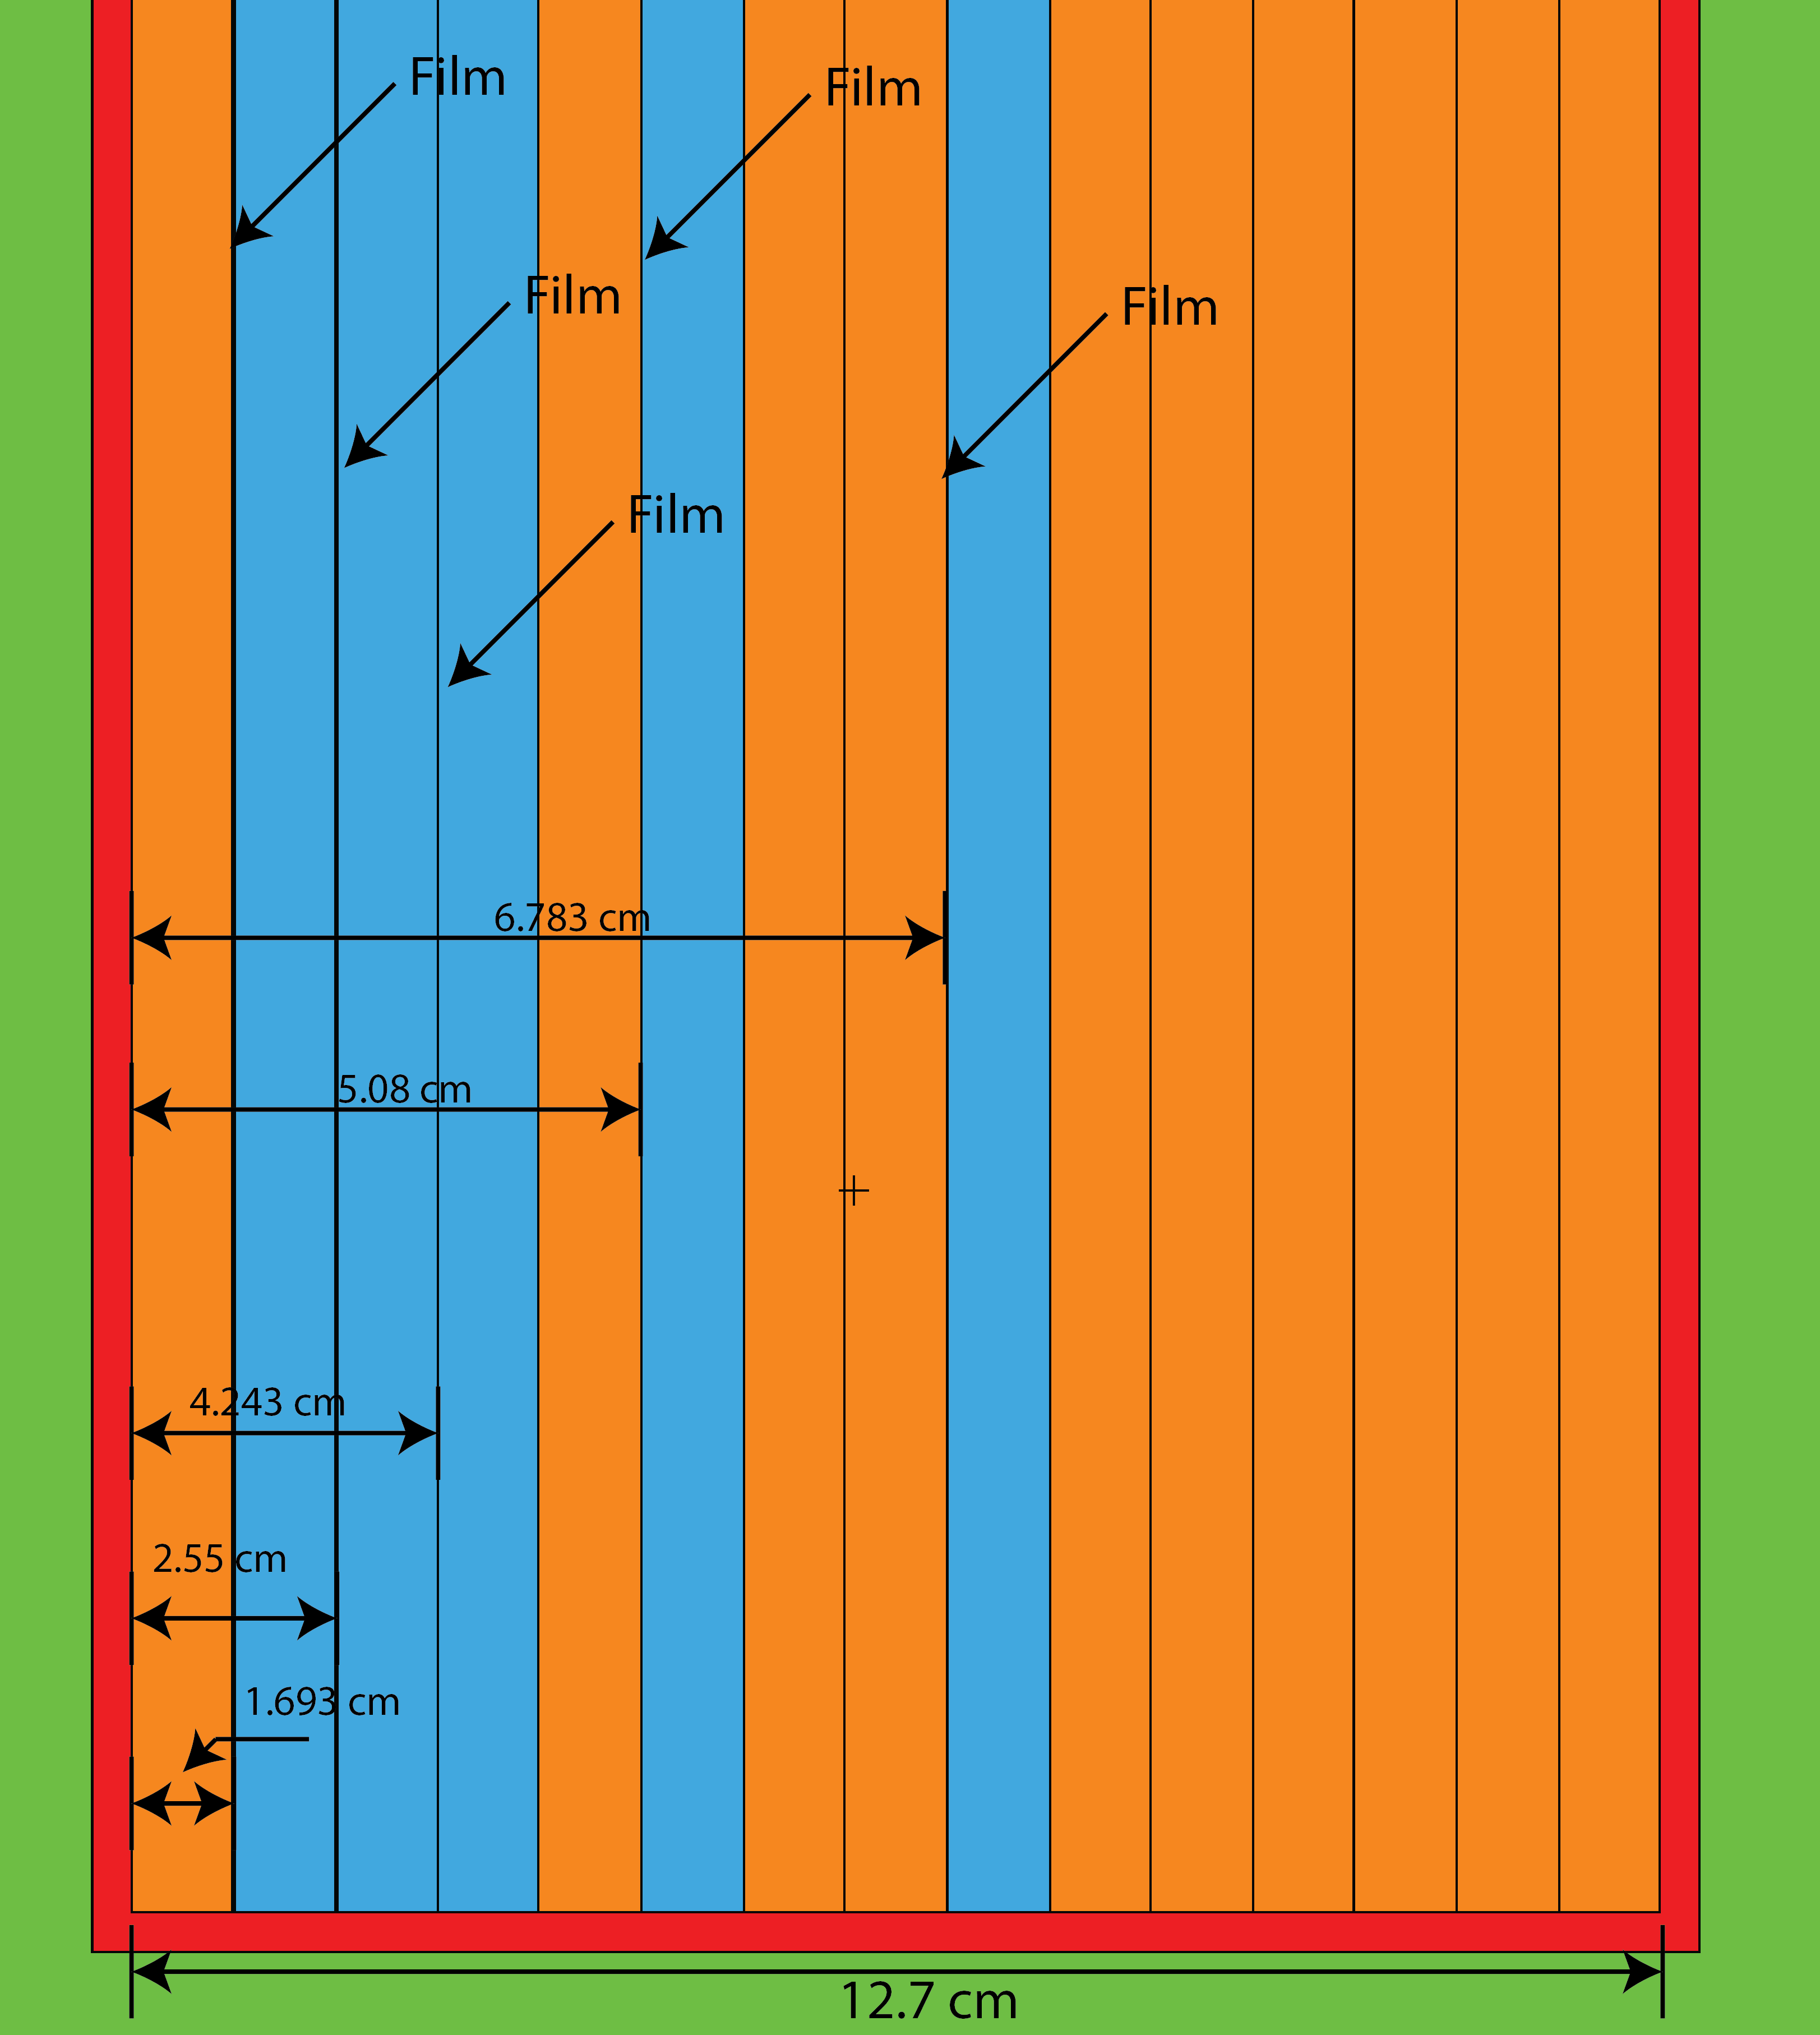
\includegraphics[width=\textwidth]{RPM8OptLayered_5cps}
    \end{subfigure}
    \caption{MCNPX rendering of layered geometry}
    \label{fig:MCNPXRendering}
\end{figure}
\end{frame}
%%%%%%%%%%%%%%%%%%%%%%%%%%%%%%%%%%%%%%%%%%%%%%%%%%%%%%%%%%%%%%%%%%%%%%%%%%
\begin{frame}[fragile]{Optimal Geometries}
\begin{table}
    %\caption[Optimal Bit String Geometries]{Genatic Algothrim Optimal Geometries}
    \centering
    \tiny
    \begin{tabular}{ p{0.75cm} | p{1cm} p{3.25cm} p{0.75cm} p{1cm} p{1cm}}
      Genome Length&Films Per Assembly&Optimal Geometry&Mass \iso[6]{Li}(g)&CPS per ng \iso[252]{Cf} & Count Rate per Mass \iso[6]{Li} (cps/g) \\
      \hline
      \hline
      3&4&\verb+010+&16.75&2.93&0.175 \\
      4&4&\verb+0100+& & & \\
      5&3&\verb+01000+&12.56&2.89&0.230 \\
      6&3&\verb+010000+&12.56&2.88&0.230 \\
      7&3&\verb+0100000+&12.56&2.84&0.226 \\ 
      10&3&\verb+0100000000+&12.56&2.68&0.214 \\
      10&3&\verb+0010000000+&12.56&2.93&0.233 \\
      10&3&\verb+0001000000+&12.56&2.95&0.235 \\
      13&2&\verb+00010010000000+&16.75&3.88&0.232 \\
      13&2&\verb+00100010000000+&16.75&3.90&0.233 \\
      13&2&\verb+00100100000000+&16.75&3.87&0.231 \\
      26&1&\verb+00000110110000000010000000+&20.94&4.33&0.206 \\
      26&1&\verb+00001010001000100000000000+&16.75&4.20&0.251 \\
    \end{tabular}
\end{table}
\end{frame}
